\documentclass[11pt,a4paper]{article}

\usepackage{mynotes}

\graphicspath{ {img/} }

\addbibresource{tls.bib}

\usepackage{makecell}
     
% Variables
\newcommand{\rawpt}{2.9e+08}
\newcommand{\voxelpt}{4.5e+07}
\newcommand{\subpt}{2.1e+07}

\newcommand{\hemiCor}{$r$(195) = 0.89, p<0.001}

\newcommand{\perIndet}{0.2}


\title{Species diversity and stand structure as drivers of canopy complexity in southern African woodlands}
\author{John L. Godlee}
\date{\today}

\begin{document}

\maketitle{}

\linenumbers

\begin{abstract}
Atmospheric CO\textsubscript{2} enrichment and human-induced climate change are expected to drive woody encroachment and an increase in tree cover across African savannas, with consequences for ecosystem function, particularly related to carbon dynamics. The patch dynamics of savanna-woodland mosaics are complex however, as woody growth is mediated by seasonal fire that is itself driven by woody canopy structure. It is unclear how variation in existing tree species composition and stand structure in this ecosystem affects canopy structure, and how this might determine vegetation dynamics. Here, I conducted the first study of canopy structure using terrestrial LiDAR in southern African savannas, at sites in Angola and Tanzania, to explore relationships between tree species diversity, stand structure, and canopy structure. I found that \todo{WHAT}
\end{abstract}

\section{Introduction}

% Woody encroachment and ecological change
Atmospheric CO\textsubscript{2} enrichment, coupled with climate change and changing disturbance regimes, is expected to drive woody encroachment, i.e. proliferation of trees in previously non-wooded areas, and woody thickening, i.e. increased growth of trees in currently wooded areas, across the savanna biome over the coming century \citep{Criado2020, Stevens2016, Mitchard2013}. As atmospheric CO\textsubscript{2} concentrations increase, C\textsubscript{3} trees are expected to gain a competitive edge over C\textsubscript{4} grasses due to differences in photosynthetic pathway \citep{Buitenwerf2012}, with cascading effects on canopy cover, grass growth, and therefore disturbance regime \citep{Bond2012}. If realised, woody encroachment and thickening will have significant effects on the global carbon cycle, as more CO\textsubscript{2} is stored as woody biomass, as well as myriad other effects on ecosystem structure \citep{Donohue2013}. Indeed, tropical savannas have been identified as the fastest increasing component of the terrestrial carbon sink \citep{Sitch2015}. Previous studies however, have reported wide variation in rates of woody encroachment and thickening \citep{Mitchard2013}, particularly in disturbance-prone savannas such as miombo woodlands in southern Africa \citep{Lewis2009}, and it is unclear how the fertilisation effect of atmospheric CO\textsubscript{2} enrichment will interact other ecosystem properties to alter vegetation \citep{Korner2017, Reich2014}.

% Southern African woodlands 
Savanna vegetation is defined by the coexistence of trees and grasses \citep{Scholes1997}. In the tropical mesic savannas of southern Africa, disturbance by fire and herbivory are the main limitations on tree cover, preventing the competitive exclusion of shade-sensitive C\textsubscript{4} grasses where climatic conditions would otherwise allow for closed canopy forest \citep{Sankaran2005}. C\textsubscript{4} grasses also provide the main fuel source for seasonal fires in these savannas \citep{Frost1996}, producing a positive feedback where an increase in tree cover reduces grass fuel load, reducing fire frequency and intensity, increasing tree cover, and so on \citep{Staver2015}. As such, even small perturbations in tree cover can lead to large changes in vegetation structure if critical thresholds of tree cover are crossed \citep{Hirota2011}. Previous research has sought to identify environmental factors which affect tree cover and its responses to atmospheric CO\textsubscript{2} enrichment, but few have considered the functional role of the existing tree community and its effect on ecosystem processes.

% Crown complementarity
Canopy structure describes the spatial distribution of tree canopy foliage \citep{Lowman2004}. Canopy structural complexity, i.e. the spatial heterogeneity of foliage distribution within the canopy, has been linked to increased net ecosystem productivity \citep{Hardiman2011,Chen2012,Law2001,Baldocchi2001,Morin2015}, increased resilience of productivity \citep{Pretzsch2014}, reduced understorey light penetration \citep{Scheuermann2018, Fotis2018}, and greater moderation of understorey micro-climate \citep{Wright2017}. Furthermore, in temperate and boreal forests, functional differences among coexisting tree species in their vertical and horizontal canopy occupation provide a link between species diversity, canopy structural complexity and canopy density, with canopy structure constituting a mechanism for observed positive biodiversity-ecosystem function effects in wooded ecosystems \citep{Pretzsch2014, Barry2019}. In tropical savannas, tree species diversity might therefore influence ecosystem-level woody thickening in response to elevated atmospheric CO\textsubscript{2}, where diverse tree communities are less limited by competition due to niche separation, and can more effectively increase foliage density and reduce understorey light penetration, excluding grass and thus reducing disturbance. 

% Stand structure
As well as the species diversity of trees, the spatial distribution and relative size of trees, i.e. stand structure, is also expected to affect canopy structural complexity \citep{Stark2015}. Heterogeneity in tree size, whether a result of species diversity, disturbance history or some other factor, is expected to increase canopy complexity and canopy density as individuals of different sizes occupy different parts of the vertical canopy space \citep{Panzou2020}, and may differ in light requirements \citep{CharlesDominique2018}. Additionally, clustering of individuals in space is expected to increase canopy structural heterogeneity across the wider savanna landscape, but ultimately decrease total foliage density due to an increase in competitive interactions \citep{Dohn2017}. Clustering may occur as a result of disturbance history, or as a result of strong facilitation effects among individuals in stressful environments \citep{Ratcliffe2017}. More diverse communities may allow more dense clustering, as differences in canopy occupancy among species can reduce competition, meaning that diversity may reduce the negative effect of disturbance on tree cover \citep{}.

% Species composition
Functional differences among floristic types of savanna may also drive variation in canopy structure, irrespective of species diversity. Some savanna trees form denser canopies than others, as a result of variation in leaf size and branch architecture. Previous studies have compared the branch architecture of ex-Acacia and miombo archetypal tree species. While ex-Acacia species tend to inhabit drier, heavily grazed or seasonally flooded areas, miombo species tend to inhabit dystrophic wetter areas structured heavily by fire  \citep{Ribeiro2020}. These studies have shown that ex-Acacia species develop sparser canopies, cagey branch architecture, and wider spreading crowns, while miombo species develop thicker canopies and can grow to large trees \citep{Mugasha2013, Archibald2003, Privette2004}. Under identical stem densities, miombo woodland species may therefore exclude grass more effectively. 

% LiDAR
Canopy structure is multi-dimensional and has previously been explained using a plethora of simple metrics that originated in forest and community ecology \citep{Kershaw2017}. Assessments of canopy structure have most often modelled tree canopies as a series of ellipses (2D), ellipsoids or cones (3D) based on field measurements with measuring tapes \citep{Jucker2015}, or used surrogate proxies for 3D canopy structure due to its inherent complexity \citep{Seidel2011}. Measurements of this kind are time consuming and yet remain an over-simplification of canopy structure. Alternatively, canopy cover is often measured using indirect optical methods which partition sky from canopy material, i.e. with hemispherical photography or the commonly used LAI-2000, providing a 2D representation of the canopy but lacking information on vertical canopy structure \citep{Jonckheere2004}. In recent years, particularly in temperate and boreal forests, LiDAR (Light Detection And Ranging) has emerged as a suitable technology for rapidly and precisely assessing canopy structure in 3D, conserving information on 3D structure of the calibre that is required to understand it's complexities \citep{Muir2018, Calders2020}. In tropical savannas, very few studies have used terrestrial LiDAR for vegetation analyses, and in southern Africa all existing studies have been located the the Skukuza Flux Tower in Kruger National Park, South Africa \citep{Muumbe2021}. Pioneering work describing the ecology of southern African savannas placed large emphasis on canopy structural diversity as a mediator of ecosystem function \citep{Solbrig1996}, but much of that understanding of savanna vegetation structure was derived from traditional mensuration methods. Using terrestrial LiDAR to measure canopy structure in southern African savannas therefore offers a unique chance to validate accepted theory and describe differences in ecosystem structure among savanna vegetation types in finer detail than previously possible.

% In this study
In this study I applied terrestrial LiDAR techniques to woodland-savanna mosaics at two sites in southern Africa, with the aim of increasing our understanding of how various metrics of tree canopy structural complexity relate to tree neighbourhood diversity and stand structure. I aim to develop our understanding of how biotic ecosystem properties in savannas might mediate responses to atmospheric CO\textsubscript{2} enrichment and climate change. I hypothesise that neighbourhoods with greater tree diversity and greater structural diversity allow greater canopy complexity, and foliage density. Thus, more diverse savannas might more effectively increase growth under elevated atmospheric CO\textsubscript{2} and are more likely to experience woody thickening through their greater occupation of environmental niche space. I also consider the functional differences among tree species in these communities and assess how combinations of these functional groups affect canopy structure and understorey light environment.

\section{Materials and methods}

\subsection{Study sites}

Field measurements were conducted at two sites, the first in Bicuar National Park, southwest Angola (S15.1$^\circ$, E14.8$^\circ$), and the second in and around Mtarure Forest Reserve, southeast Tanzania (S9.0$^\circ$, E39.0$^\circ$) (\autoref{map}). At each site, 1 ha (100x100 m) plots were located in areas of savanna-woodland vegetation, across a gradient of stem density and range of savanna floristic archetypes. In Angola, 15 plots were sampled, while in Tanzania, seven were sampled following the curtailment of fieldwork due to COVID-19 travel restrictions. Fieldwork was conducted between February and April at both sites, during the peak growth period of each site in order to capture the greatest foliage volume in the canopy.

\begin{figure}
	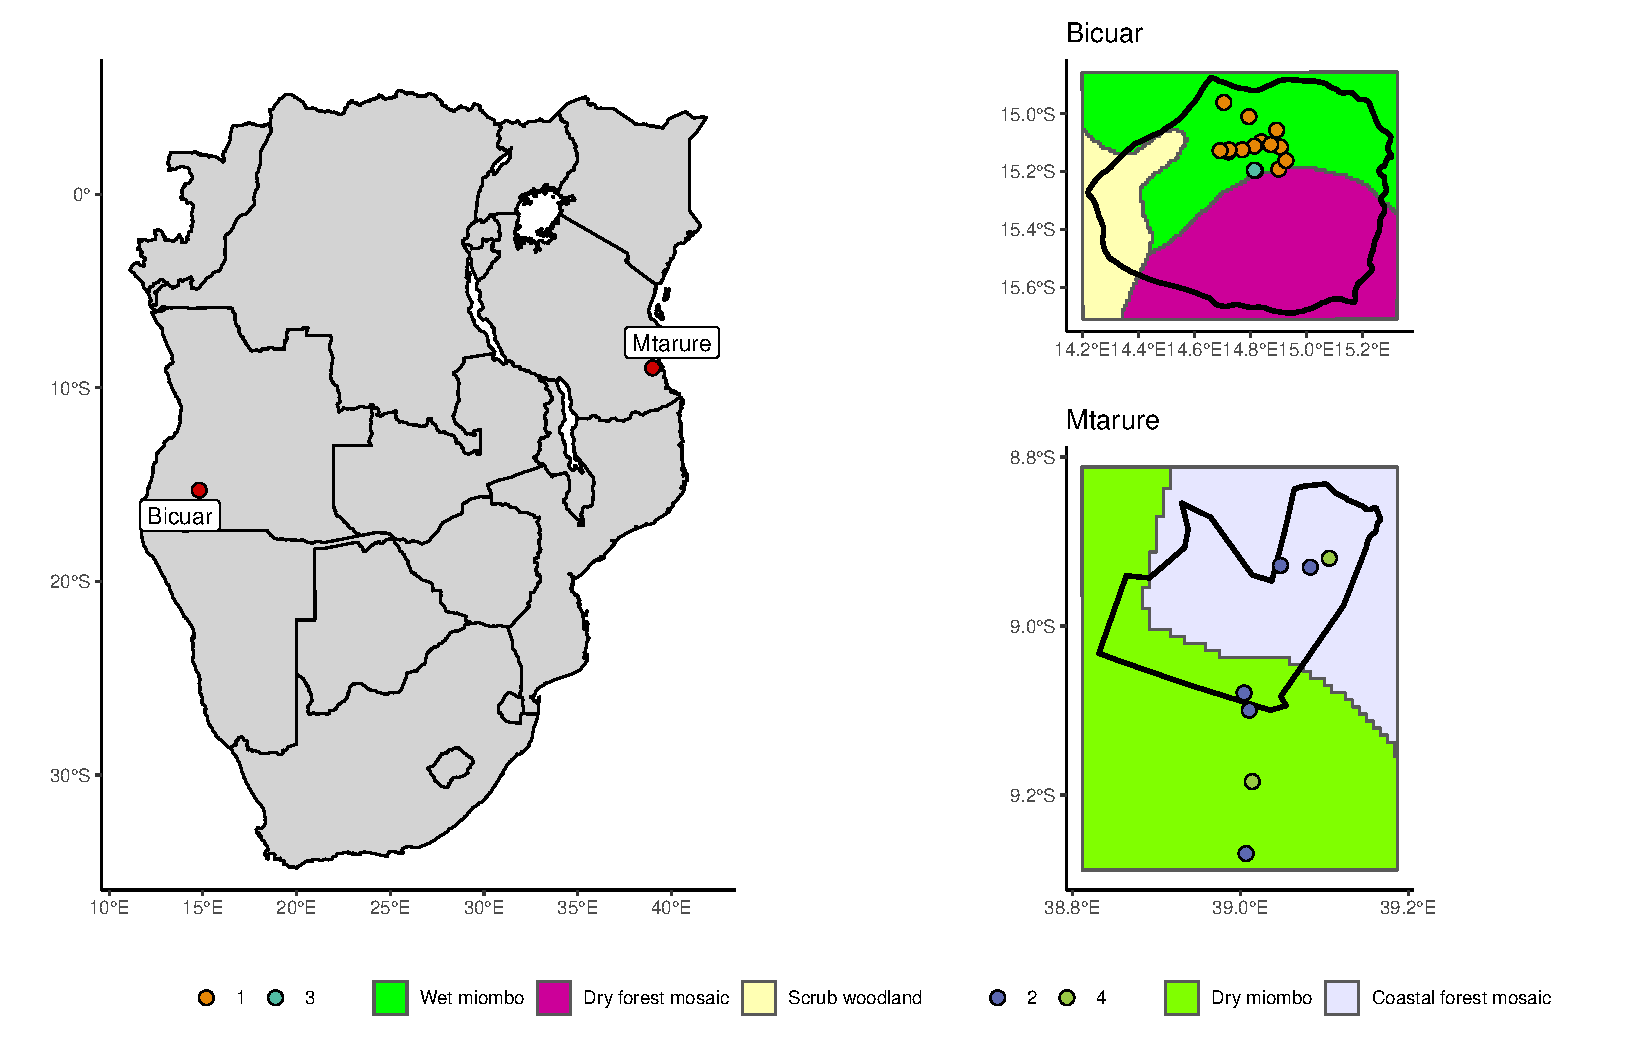
\includegraphics[width=\linewidth]{map}
	\caption{Location of study sites within southern Africa (left), and of 1 ha plots within each site (right). The black outlines in each site map denote the boundaries of protected areas which encompass the majority of study sites, Bicuar National Park in Angola (top), and Mtarure Forest Reserve in Tanzania (bottom). The background of each site map is a re-classified version of White's vegetation map \citep{White1983}. Note that all maps are on different scales.}
	\label{map}
\end{figure}

\subsection{Field measurements}

Within each 1 ha plot we identified each woody stem >5 cm stem diameter to species, measured stem diameter (Diameter at Breast Height - 1.3 m) and recorded stem location within the plot using tape measures. Each 1 ha plot was further subdivided into nine 10 m diameter circular subplots arranged in a regular grid, with a 15 m buffer from the plot edge and 35 m between subplots. For each subplot, we recorded the distance and direction from the subplot centre of each stem >5 cm diameter with canopy material inside the subplot. Within each subplot, a variable number of scans were recorded using a Leica HDS6100 phase-shift Terrestrial Laser Scanner (TLS). The number and position of scans within a subplot was determined by the arrangement of canopy material in the subplot, to minimise shadows within the canopy of the subplot, and to maximise canopy penetration. The number of scans per subplot ranged between one and five across both sites. Extended field methods and data analysis methods are described in Chapter 6.

\subsection{Data analysis}

\subsubsection{TLS processing}

Point clouds from scans in each subplot were registered and unified using Leica Cyclone (version 9.1), using five reflective cross targets visible to all scans. Point clouds were voxelised to cubic voxel sizes of different sizes depending on the application of the data. For subplot height profile estimation and gap fraction we used 5 cm\textsuperscript{3} voxels, and for whole plot canopy rugosity we used 50 cm\textsuperscript{3} voxels. Voxels were classified as `filled' if they intersected one or more points. Variation in voxel size reflects the spatial scale of each analysis, and is bounded by the beam divergence of the scanner over longer distances \citep{}. Choosing voxels that are too small can result in pock-marked representations of surfaces that are especially problematic when calculating larger scale canopy structure metrics such as canopy top roughness, while voxels that are too large can result in an over-estimation of plant volume when estimating canopy foliage density at the subplot scale \citep{Seidel2012, Cifuentes2014}. We used the noise reduction algorithm from \citet{Rusu2008} to discard points based on mean nearest neighbour distances, with a mean number of neighbours of eight, and a standard deviation threshold of 1.96. This effectively removed `ghost points' produced by partial beam interceptions and also removed many erroneous returns caused by airborne dust particles, which was common at our study sites. Raw points clouds for each subplot had a mean of \textasciitilde{}\rawpt{} points, \textasciitilde{}\voxelpt{} points after voxelisation to 5 cm\textsuperscript{3}, and \textasciitilde{}\subpt{} points after noise reduction. Ground points were classified using the Progressive Morphological Filter (PMF) from \citet{Zhang2003}. Point cloud height was reclassified height based on this revised ground layer by measuring the vertical distance between the nearest ground point and each point.

At the subplot level, we used ray-tracing to estimate canopy closure, i.e. the proportion of the sky hemisphere occluded by plant material at the subplot centre from multiple TLS scans. Hemispherical images were created using the POV-Ray ray-tracing software \citep{Povray2004}. Filled voxels were represented as matt black cubes filling the voxel volume, with a white sky box and no light source. A `camera' with a 180\textdegree{} fisheye lens was placed at the subplot centre within POV-Ray, at a height of 1.8 m pointing directly upwards. The images produced by POV-Ray were analysed using Hemiphot \citep{HemiPhot} to estimate canopy closure as the proportion of pixels filled by canopy material. Canopy closure estimates from the TLS were validated with hemispherical photographs taken at the same location and processed using the same method in Hemiphot, and compared using Pearson's correlation (\hemiCor{}). The Effective Number of Layers (ENL) measures subplot canopy complexity and was calculated as the Shannon entropy of foliage density among 50 cm height bins within each subplot. The uniformity of foliage distribution was calculated by fitting a linear model to the cumulative foliage density profile, then extracting the standard error on the slope estimate of this linear model. Total foliage density was calculated as the area under the curve of the foliage height profile. 

At the plot level, canopy complexity was measured by two metrics. Canopy top roughness was measured as the standard deviation of canopy height across the plot. Canopy rugosity was measured according to \citet{Hardiman2011}, as the standard deviation of vertical and horizontal foliage density within 0.5 m cubic bins. We also estimated plot-level canopy closure by calculating the mean of the canopy closure values from each subplot.

\subsubsection{Stand structure}

For each subplot, we calculated an adapted version of the Hegyi index to estimate crowding, as an alternative to stem density which does not adequately capture crowding at small spatial scales, when only a small number of trees are included in the sample \citep{Hegyi1974}. To estimate subplot structural diversity we calculated the coefficient of variation of stem diameter as a measure of the heterogeneity of tree size in the neighbourhood. 

At the plot level, we estimated the regularity of species spatial distribution using the spatial mingling index \citep{Gadow2002}. We also measured the uniformity of whole plot stem distribution using the winkelmass, which measures the spatial clustering of stems \citep{Gadow2002}. Finally, we calculated plot level stem density.

\subsubsection{Statistical analysis}

To describe variation in species composition among plots, we conducted Non-metric Multi-dimensional Scaling (NMDS) analysis on genus-level basal area weighted abundance in each plot. We excluded stems that could not be identified to genus from this analysis, which accounted for \perIndet{}\% of the total basal area recorded. Four distinct vegetation types were identified, two from each site (\autoref{clust_summ}). 

Linear mixed effects models tested the effects of tree species diversity and stand structural diversity on canopy complexity. Mixed models were used to account for the nested sampling design of subplots within plots and plots within vegetation types. Models were conducted at both the subplot and plot level. Subplot models included random effects for plot nested within vegetation type, while plot level models included random effects for vegetation type only. Separate models were fitted for each canopy complexity metric, resulting in four models at the subplot level and four models at the plot level. We compared effect sizes among fixed effects in each model, and also compared AIC values and Akaike weights of models with different combinations of fixed effects to determine which diversity and structural metrics best explained variation in each canopy complexity metric. The ex-Acacia vegetation type in Tanzania was represented by only two plots and so could not be included in plot-level statistical models due to lack of replication. 

To test whether tree species diversity may influence canopy complexity indirectly through its effect on stand structure, we conducted a path analysis using the \texttt{piecewiseSEM} R package \citep{piecewiseSEM}. The path analysis investigated the direct effect of plot species richness on mean plot canopy closure, as well as the indirect effect of richness on canopy closure via the coefficient of variation of basal area, with random intercept terms for each vegetation type. Again, the ex-Acacia vegetation type could not be included in this model due to lack of replication.

% latex table generated in R 4.1.0 by xtable 1.8-4 package
% Tue Aug 10 12:19:25 2021
\begin{table}[h]
\centering
\caption{Description of the vegetation type clusters identified using the Ward algorithm, based on basal area weighted genus abundances. AGB = Above-Ground woody Biomass. Species richness, stem density and AGB are reported as the median among plots, with the interquartile range in parentheses.} 
\label{clust_summ}
\begin{tabular}{lS[table-format=2.0]rrr}
  \toprule
{Cluster} & {N sites} & {Richness} & {Stem density} & {AGB} \\ 
  \midrule
1 & 12 & 17(2) & 642(194) & 41( 8.4) \\ 
  2 & 5 & 23(4) & 411(137) & 72(11.9) \\ 
  3 & 3 &  6(1) & 196( 55) & 77( 7.3) \\ 
  4 & 2 & 12(2) & 288( 73) &  9( 0.2) \\ 
   \bottomrule
\end{tabular}
\end{table}



% latex table generated in R 4.1.0 by xtable 1.8-4 package
% Mon Aug 16 12:52:51 2021
\begin{table}[]
\centering
\caption{Floristic description of the vegetation type clusters. Dominant species are the most abundant individuals across all plots per cluster. Indicator species are derived from Dufr\^{e}ne-Legendre indicator species analysis with the three highest indicator values.} 
\label{indval}
\begin{tabular}{crrS[table-format=1.2]}
  \toprule
{Cluster} & {Dominant species} & {Indicator species} & {Indicator value} \\ 
  \midrule
1 & Julbernardia paniculata & Strychnos spinosa & 0.83 \\ 
  1 & Burkea africana & Combretum collinum & 0.74 \\ 
  1 & Combretum collinum & Julbernardia paniculata & 0.70 \\ 
   \midrule
2 & Diplorhynchus condylocarpon & Pteleopsis myrtifolia & 1.00 \\ 
  2 & Pseudolachnostylis maprouneifolia & Diplorhynchus condylocarpon & 0.89 \\ 
  2 & Gymnosporia senegalensis & Pseudolachnostylis maprouneifolia & 0.81 \\ 
   \midrule
3 & Baikiaea plurijuga & Baikiaea plurijuga & 0.94 \\ 
  3 & Baphia massaiensis & Baphia massaiensis & 0.83 \\ 
  3 & Philenoptera nelsii & Philenoptera nelsii & 0.45 \\ 
   \midrule
4 & Combretum apiculatum & Vachellia nilotica & 0.99 \\ 
  4 & Burkea africana & Combretum apiculatum & 0.70 \\ 
  4 & Bauhinia petersiana & Senegalia polyacantha & 0.62 \\ 
   \bottomrule
\end{tabular}
\end{table}



\section{Results}

\subsection{Description of vegetation types}

Indicator species analysis showed that the four identified vegetation types constitute common southern African savanna floristic archetypes. Cluster 1, found in Bicuar National Park contains typical miombo species from the Detarioideae subfamily, such as \textit{Julbernardia paniculata}. This vegetation type is the most common in our study, with 12 plots. Cluster 1 has the highest stem density, but lower AGB than Clusters 2 or 3, which contain larger individuals. Cluster 2, found in Mtarure is dominated by \textit{Pteleopsis myrtifolia} another large canopy forming tree species that is common in mixed miombo woodland found on the east coast of southern Africa. Cluster 3 represents \textit{Baikiaea} woodland, found on Kalahari sands in southern Angola. It is species poor and dominated by \textit{Baikiaea plurijuga} which forms large spreading canopy trees. Other shrubby species that coppice readily such as \textit{Baphia massaiensis} are also common. Cluster 4, found in Mtarure is a type of ex-Acacia woodland, dominated by \textit{Vachellia} and \textit{Senegalia} spp. This vegetation type was not well represented in our study, with only two plots, precluding its use in plot-level statistical analyses due to lack of replication. Cluster 4 had far lower AGB than the other clusters. Differences in canopy structure among the four vegetation types are visible in canopy surface models for typical plots within each type (\autoref{veg_type_tile}). Cluster 1 shows many overlapping crowns forming a nearly contiguous canopy surface, though most trees in Cluster 1 have smaller crowns than those in Cluster 2, which also forms a nearly contiguous canopy. The largest trees in Cluster 2 grow taller and have a wider spreading canopy than those in other sites. Cluster 3 shows two distinct size classes of tree, the large \textit{Baikiaea plurijuga} forming clear isolated canopies with an inverted cone shape, and much smaller scattered shrubby individuals in the understorey. Cluster 4 shows many small shrubby individuals with irregular canopy shapes, but a greater total tree cover than Cluster 3. 

\begin{figure}
	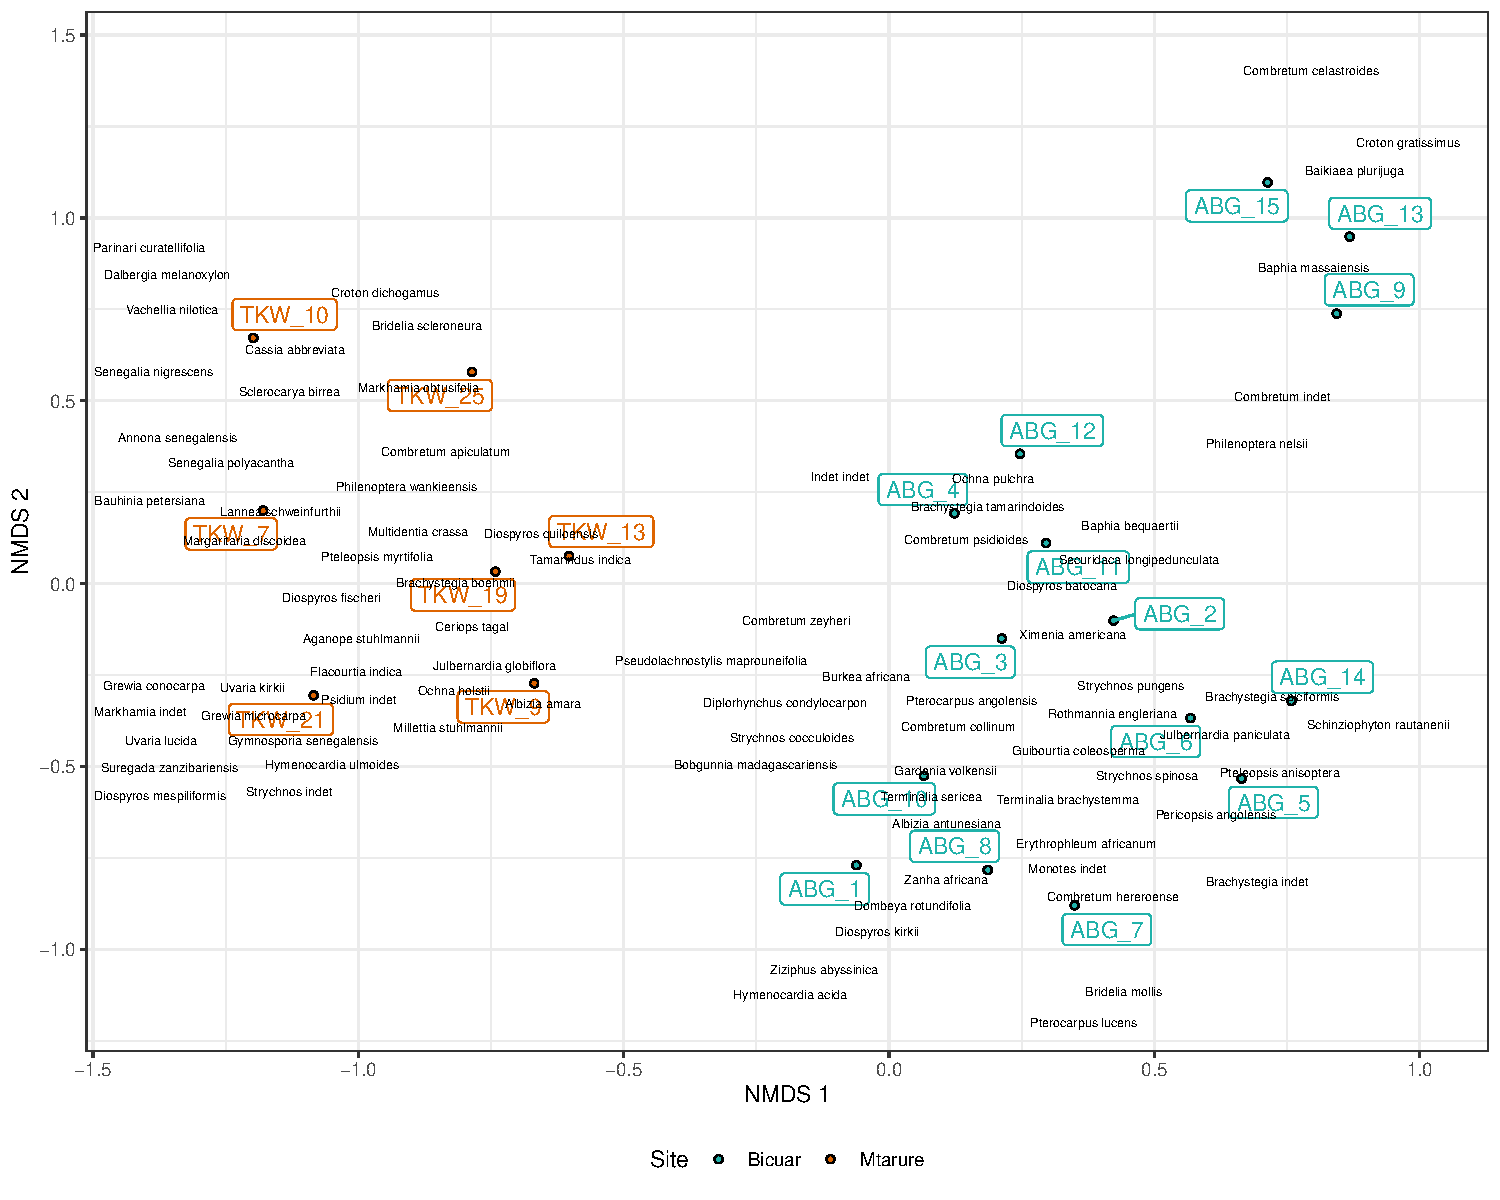
\includegraphics[width=\linewidth]{nmds}
	\caption{The first two axes of a Non-metric Multi-Dimensional Scaling (NMDS) analysis of tree species diversity in each plot. Species scores are labelled as black text, while plot scores are labelled as coloured points. Plots can be split into four principal groups: 1) B9, B13 and B15, dominated by \textit{Baikiaea plurijuga}; 2) the other Bicuar plots; 3) M2, M5, M6, and M7,dominated by \textit{Julbernardia} spp., \textit{Brachystegia} spp. and \textit{Ochna} spp.; 4) M1, M3, and M4, dominated by \textit{Senegalia} spp. and \textit{Vachellia} spp..}
	\label{nmds}
\end{figure}

\subsection{Bivariate relationships}

Bivariate plots show that subplot species diversity, measured by species richness of the tree neighbourhood around each 10 m diameter subplot, appears to have weak positive effects on canopy layer diversity and total canopy closure (\autoref{subplot_canopy_bivar}). The Hegyi crowding index had strong positive effects on canopy cover as expected, and also positive effects on layer diversity and total canopy foliage density. Structural diversity, measured as the coefficient of variation of subplot basal area had a positive significant effect on layer diversity, but a negligible effect on total canopy foliage and canopy cover. The effect of Hegyi crowding on subplot canopy complexity was similar across all vegetation types. 

At the plot level, effects of species diversity and stand structure on canopy structure were more variable. Variation among vegetation types masked any meaningful inference to be drawn from most of the bivariate plots. One exception is the effect of spatial clustering of stems, measured by the winkelmass, on canopy cover, which is clearly negative. Additionally, there is a weak positive effect of coefficient of basal area on canopy surface roughness and a negative effect on whole canopy rugosity. 

Vegetation types differed greatly in their subplot and whole-plot canopy structural metrics (\autoref{plot_subplot_bivar}). Cluster 4, representing seasonally flooded ex-Acacia savanna, had a much shorter and simpler canopy, with more space between tree canopies (\autoref{veg_type_tile}). 

\begin{landscape}
\begin{figure}
	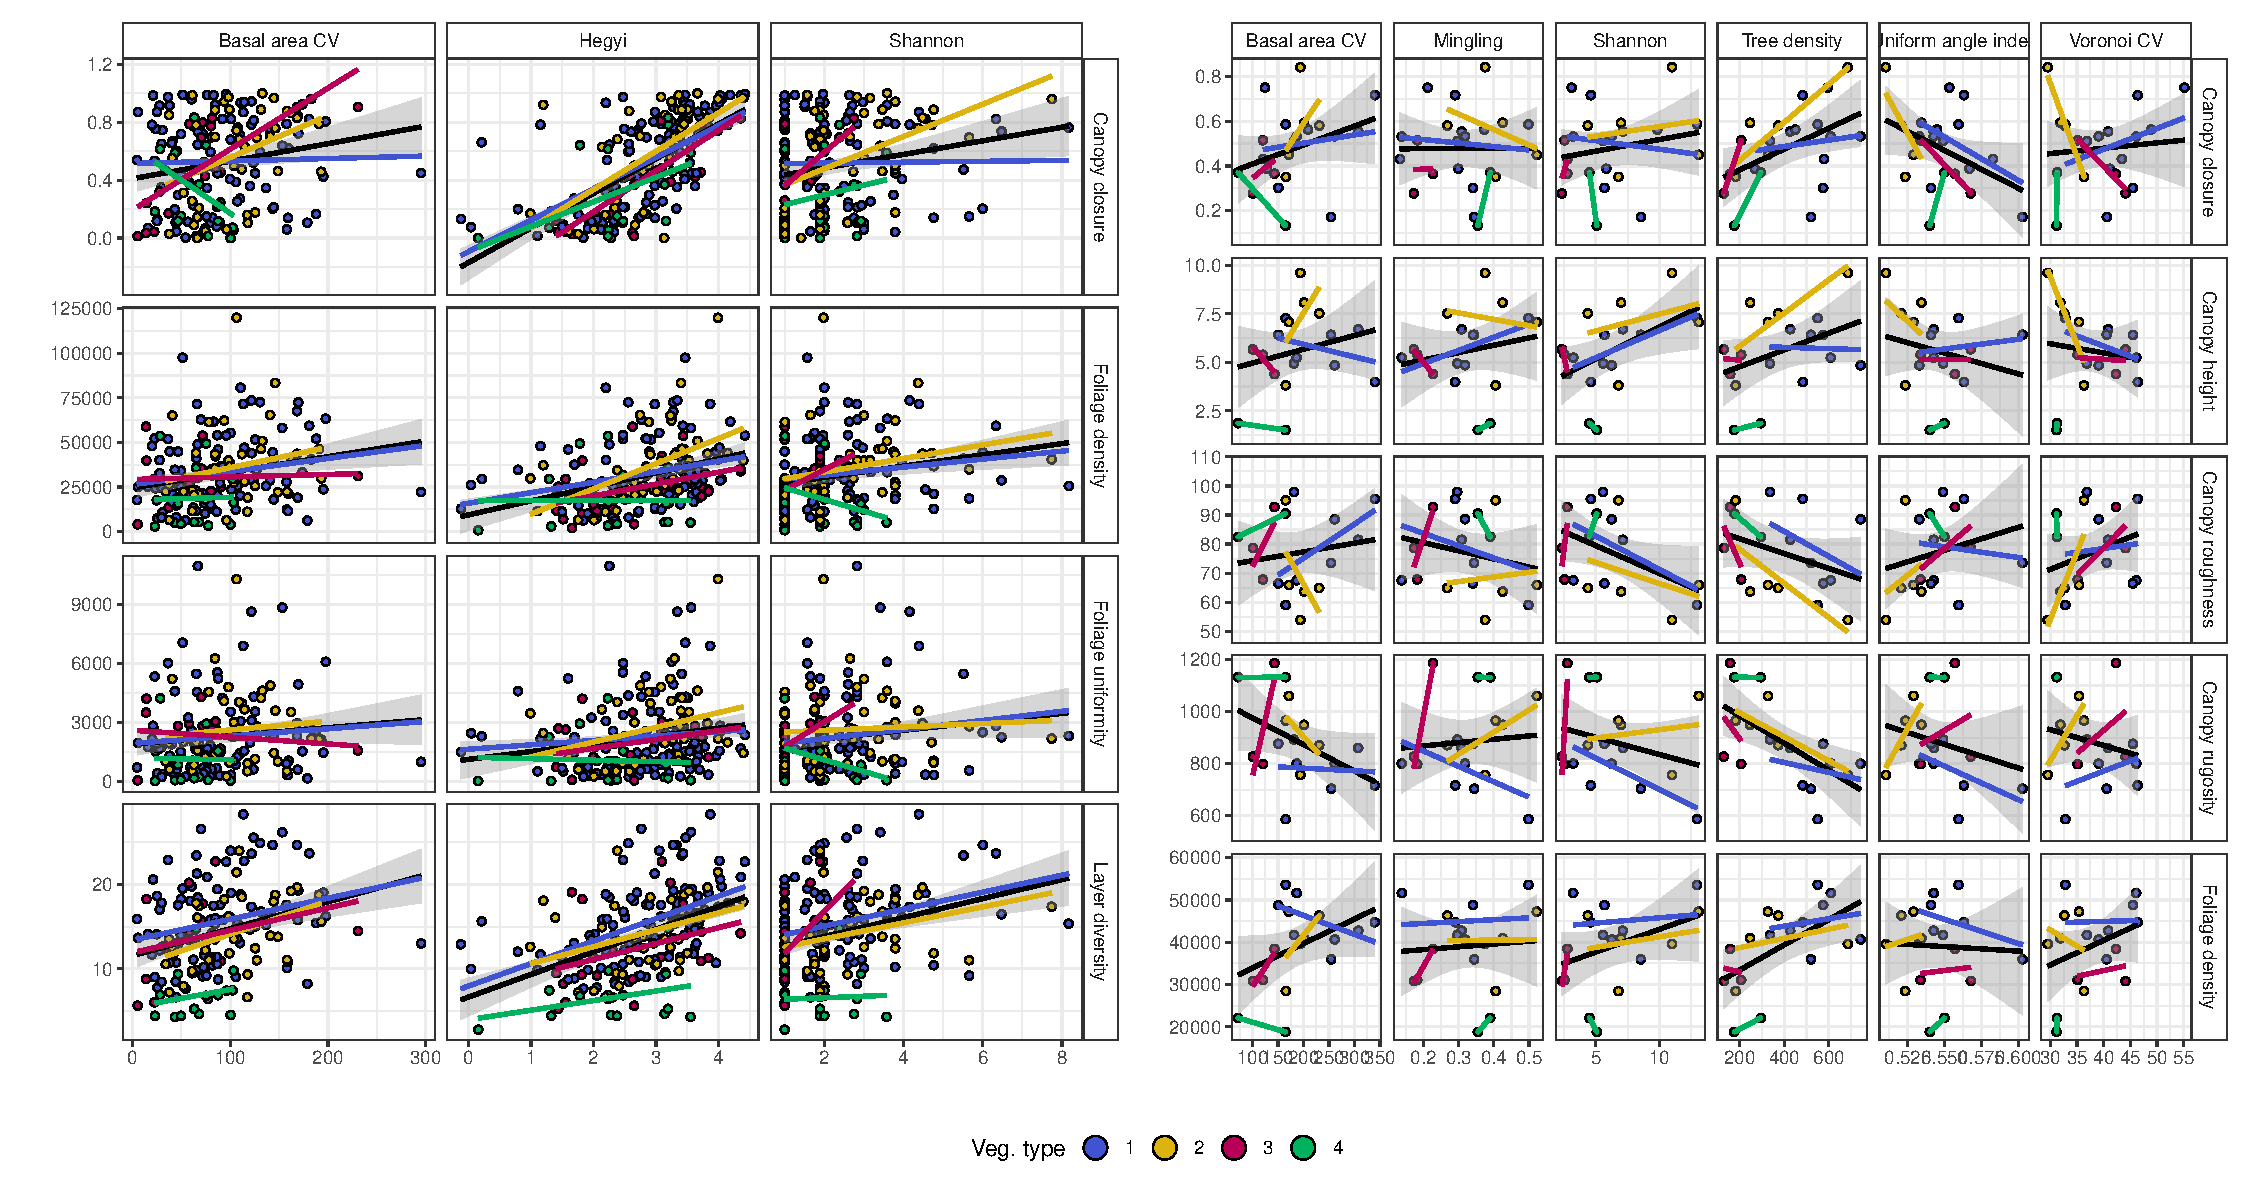
\includegraphics[width=\linewidth]{bivar}
	\caption{Bivariate relationships between diversity/stand structure metrics (x axis) and canopy structure metrics (y axis), at both the subplot level (left) and the plot level (right). Points and linear model lines of best fit are coloured by vegetation type. Black lines of best fit are linear models including all plots, with a 95\% confidence interval. See \autoref{bivar_lm_summ} for a comparison of linear model fits by vegetation type.}
	\label{subplot_canopy_bivar}
\end{figure}
\end{landscape}

\begin{figure}
	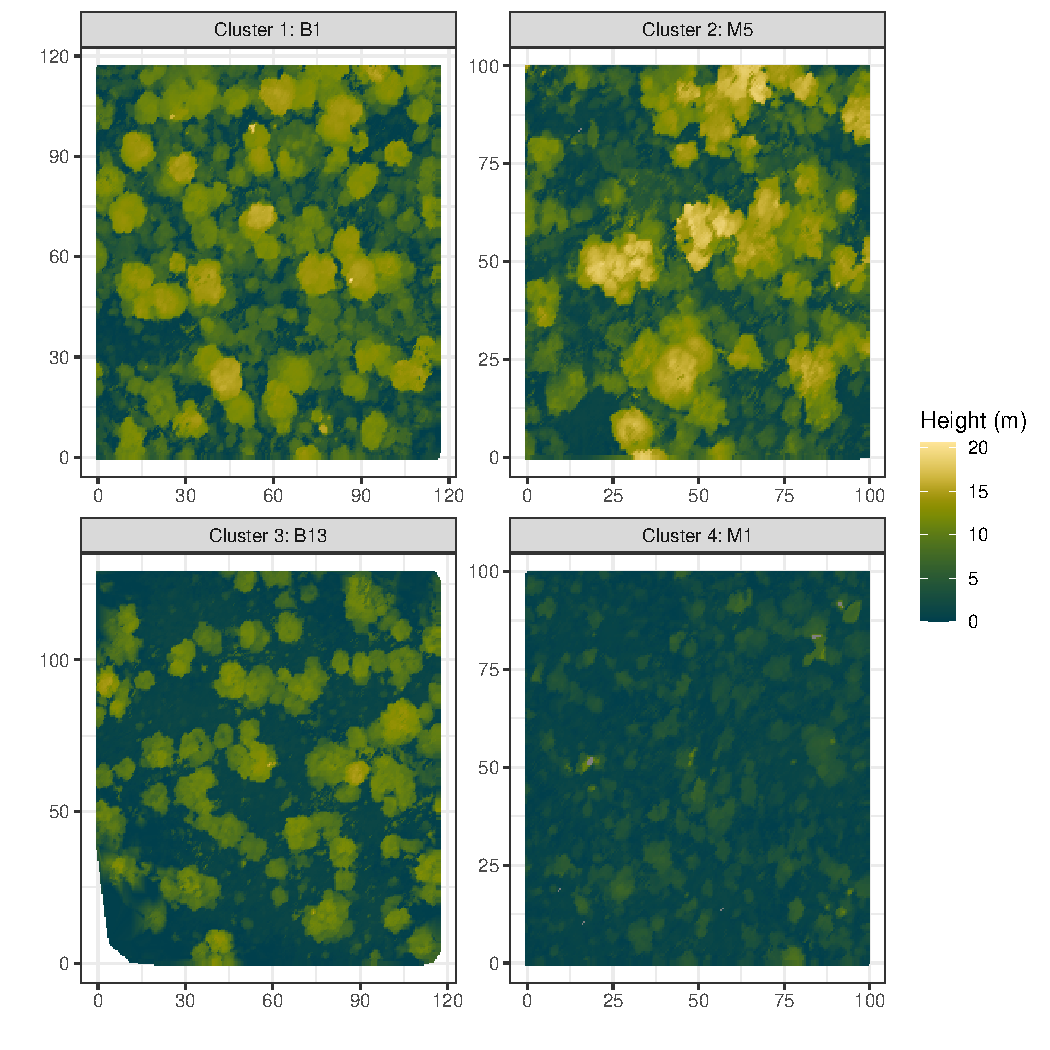
\includegraphics[width=\linewidth]{veg_type_tile}
	\caption{Representative canopy surface models for each vegetation type identified in the Non-metric Multi-dimensional Scaling (NMDS) analysis. Plot titles show the plot name and the vegetation type.}
	\label{veg_type_tile}
\end{figure}

\subsection{Subplot model selection}

Linear mixed effects models showed that species richness of the subplot neighbourhood had negligible effects on canopy structure (\autoref{height_profile_mod_rich_slopes_sites}). As seen in \autoref{subplot_canopy_bivar}, the Hegyi crowding index had strong positive effects on all measured canopy complexity metrics. Heterogeneity of stem basal area had a positive effect on layer diversity (\todo{MORE}). 

\begin{figure}
	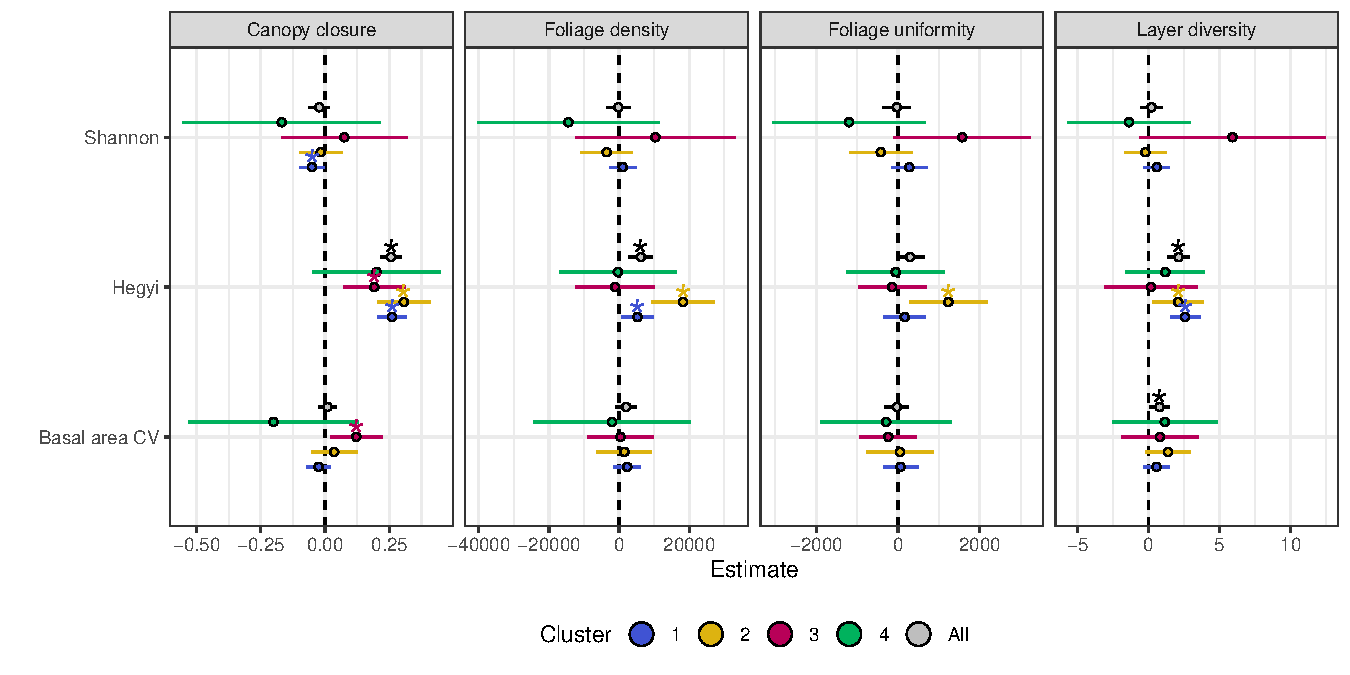
\includegraphics[width=\linewidth]{height_profile_mod_rich_slopes_sites}
	\caption{Standardized fixed effect slopes for each model of a canopy structure metric. Slope estimates are $\pm$1 standard error. Slope estimates where the interval (standard error) does not overlap zero are considered to be significant effects. Points are coloured according to site.}
	\label{height_profile_mod_rich_slopes_sites}
\end{figure}

Model selection showed that none of the best models for subplot canopy complexity metrics included species richness (\autoref{height_profile_sig_vars_dredge}). Stand structural diversity metrics were included in the best models for layer diversity and total foliage density, with the fixed effects for these models explaining 17\% and 19\% of the variation in these metrics, respectively. The random effects of vegetation type and plot identity decribed most of the variation in layer diversity and total canopy foliage density. Uniformity of foliage distribution was poorly described by all candidate models, with the best model only describing 8\% of the variation in this metric. All models were better than random effects only models according to AIC values.

% latex table generated in R 4.1.0 by xtable 1.8-4 package
% Wed Aug 11 17:43:51 2021
\begin{table}[]
\centering
\caption{Explanatory variables included in the best model for each canopy structure variable. $\Delta$AIC shows the difference in model AIC value compared to a null model which included only the hegyi crowding index and the random effects of vegetation type and plot. R\textsuperscript{2}\textsubscript{c} is the R\textsuperscript{2} of the best model, while R\textsuperscript{2}\textsubscript{m} is the R\textsuperscript{2} of the model fixed effects only.} 
\label{height_profile_sig_vars_dredge}
\begin{tabular}{lcccccc}
  \toprule
{Response} & {Hegyi} & {Richness} & {CoV basal area} & {$\Delta$AIC} & {R\textsuperscript{2}\textsubscript{c}} & {R\textsuperscript{2}\textsubscript{m}} \\ 
  \midrule
Layer diversity & \checkmark &  & \checkmark & 37.4 & 0.50 & 0.17 \\ 
  Foliage density & \checkmark &  & \checkmark & 77.7 & 0.28 & 0.19 \\ 
  Foliage uniformity & \checkmark &  &  & 37.4 & 0.12 & 0.05 \\ 
  Canopy closure & \checkmark &  &  & 104.0 & 0.63 & 0.49 \\ 
   \bottomrule
\end{tabular}
\end{table}



\subsection{Whole-plot model selection}

While species diversity had varying effects on different plot-level canopy structural metrics, the confidence intervals on these effect sizes were wide (\autoref{canopy_rough_slopes}). Richness appeared to have a positive effect on canopy height and canopy cover, but a negative effect on canopy surface roughness and rugosity. Similarly, plot total basal area had a strong positive effect on canopy height and canopy cover, and negative effects on roughness and rugosity. Structural diversity, measured by the coefficient of variation of basal area had a strong positive effect on canopy roughness. Spatially explicit measures of structural and species diversity, measured by the spatial mingling index and winkelmass, had negligible effects on all canopy structural metrics. One exception was the effect of the winkelmass, i.e. the spatial clustering of stems, on canopy cover, which was negative.

\begin{figure}
	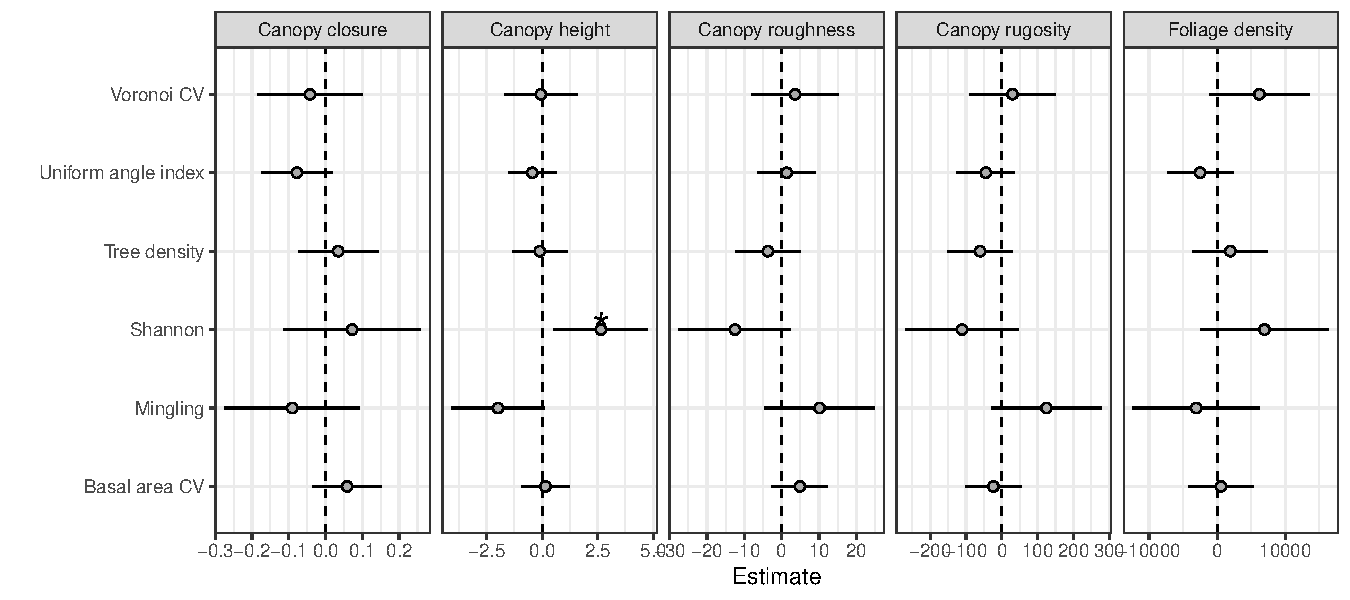
\includegraphics[width=\linewidth]{canopy_rough_slopes}
	\caption{Standardized fixed effect slopes for whole-plot canopy rugosity. Slope estimates are $\pm$1 standard error. Slope estimates where the interval (standard error) does not overlap zero are considered to be significant effects.}
	\label{canopy_rough_slopes}
\end{figure}

Model selection showed that all plot canopy complexity metrics except canopy rugosity were best modelled by a combination of basal area and either species diversity or structural diversity. 

% latex table generated in R 4.1.0 by xtable 1.8-4 package
% Mon Aug  9 15:44:59 2021
\begin{table}[H]
\centering
\begin{tabular}{rcccccccc}
  \hline
Response & Richness & Basal area & CoV basal area & Mingling & Winkelmass & $\Delta$AIC & R\textsuperscript{2}\textsubscript{c} & R\textsuperscript{2}\textsubscript{m} \\ 
  \hline
Canopy cover & \checkmark &  &  &  &  & -19.1 & 0.57 & 0.57 \\ 
  Canopy height & \checkmark & \checkmark &  &  &  & 9.0 & 0.77 & 0.77 \\ 
  Canopy roughness & \checkmark & \checkmark & \checkmark &  &  & 24.7 & 0.54 & 0.54 \\ 
  Rugosity &  & \checkmark &  &  &  & 43.7 & 0.57 & 0.35 \\ 
   \hline
\end{tabular}
\caption{Explanatory variables included in the best model for each plot-level canopy complexity metric. $\Delta$AIC shows the difference in model AIC value compared to a null model which included only the hegyi crowding index and the random effects of site and plot. R\textsuperscript{2}\textsubscript{c} is the R\textsuperscript{2} of the best model, while R\textsuperscript{2}\textsubscript{m} is the R\textsuperscript{2} of the model fixed effects only.} 
\label{canopy_sig_vars_dredge}
\end{table}



\subsection{Comparing subplot and plot measures of canopy structure}

Plot-level and subplot-level canopy structure metrics were highly correlated in many cases (\autoref{canopy_rough_slopes}). Plot canopy height especially, tended to be strongly positively correlated with subplot canopy complexity. Additionally, as canopy top roughness increases, many subplot canopy complexity and density metrics increase. In the majority of cases, both sites had similar correlations of subplot and plot measures of canopy structure, with notable exceptions for plot roughness vs. layer diversity, plot roughnesss vs. canopy closure, and plot canopy height vs. canopy closure.

Variance of plot canopy height and plot roughness was larger in Mtarure than Bicuar. The increase in variance was caused by two particularly sparse thorny savanna plots in Mtarure, M3 and M4, which had very low canopy height and roughness.

\begin{figure}
	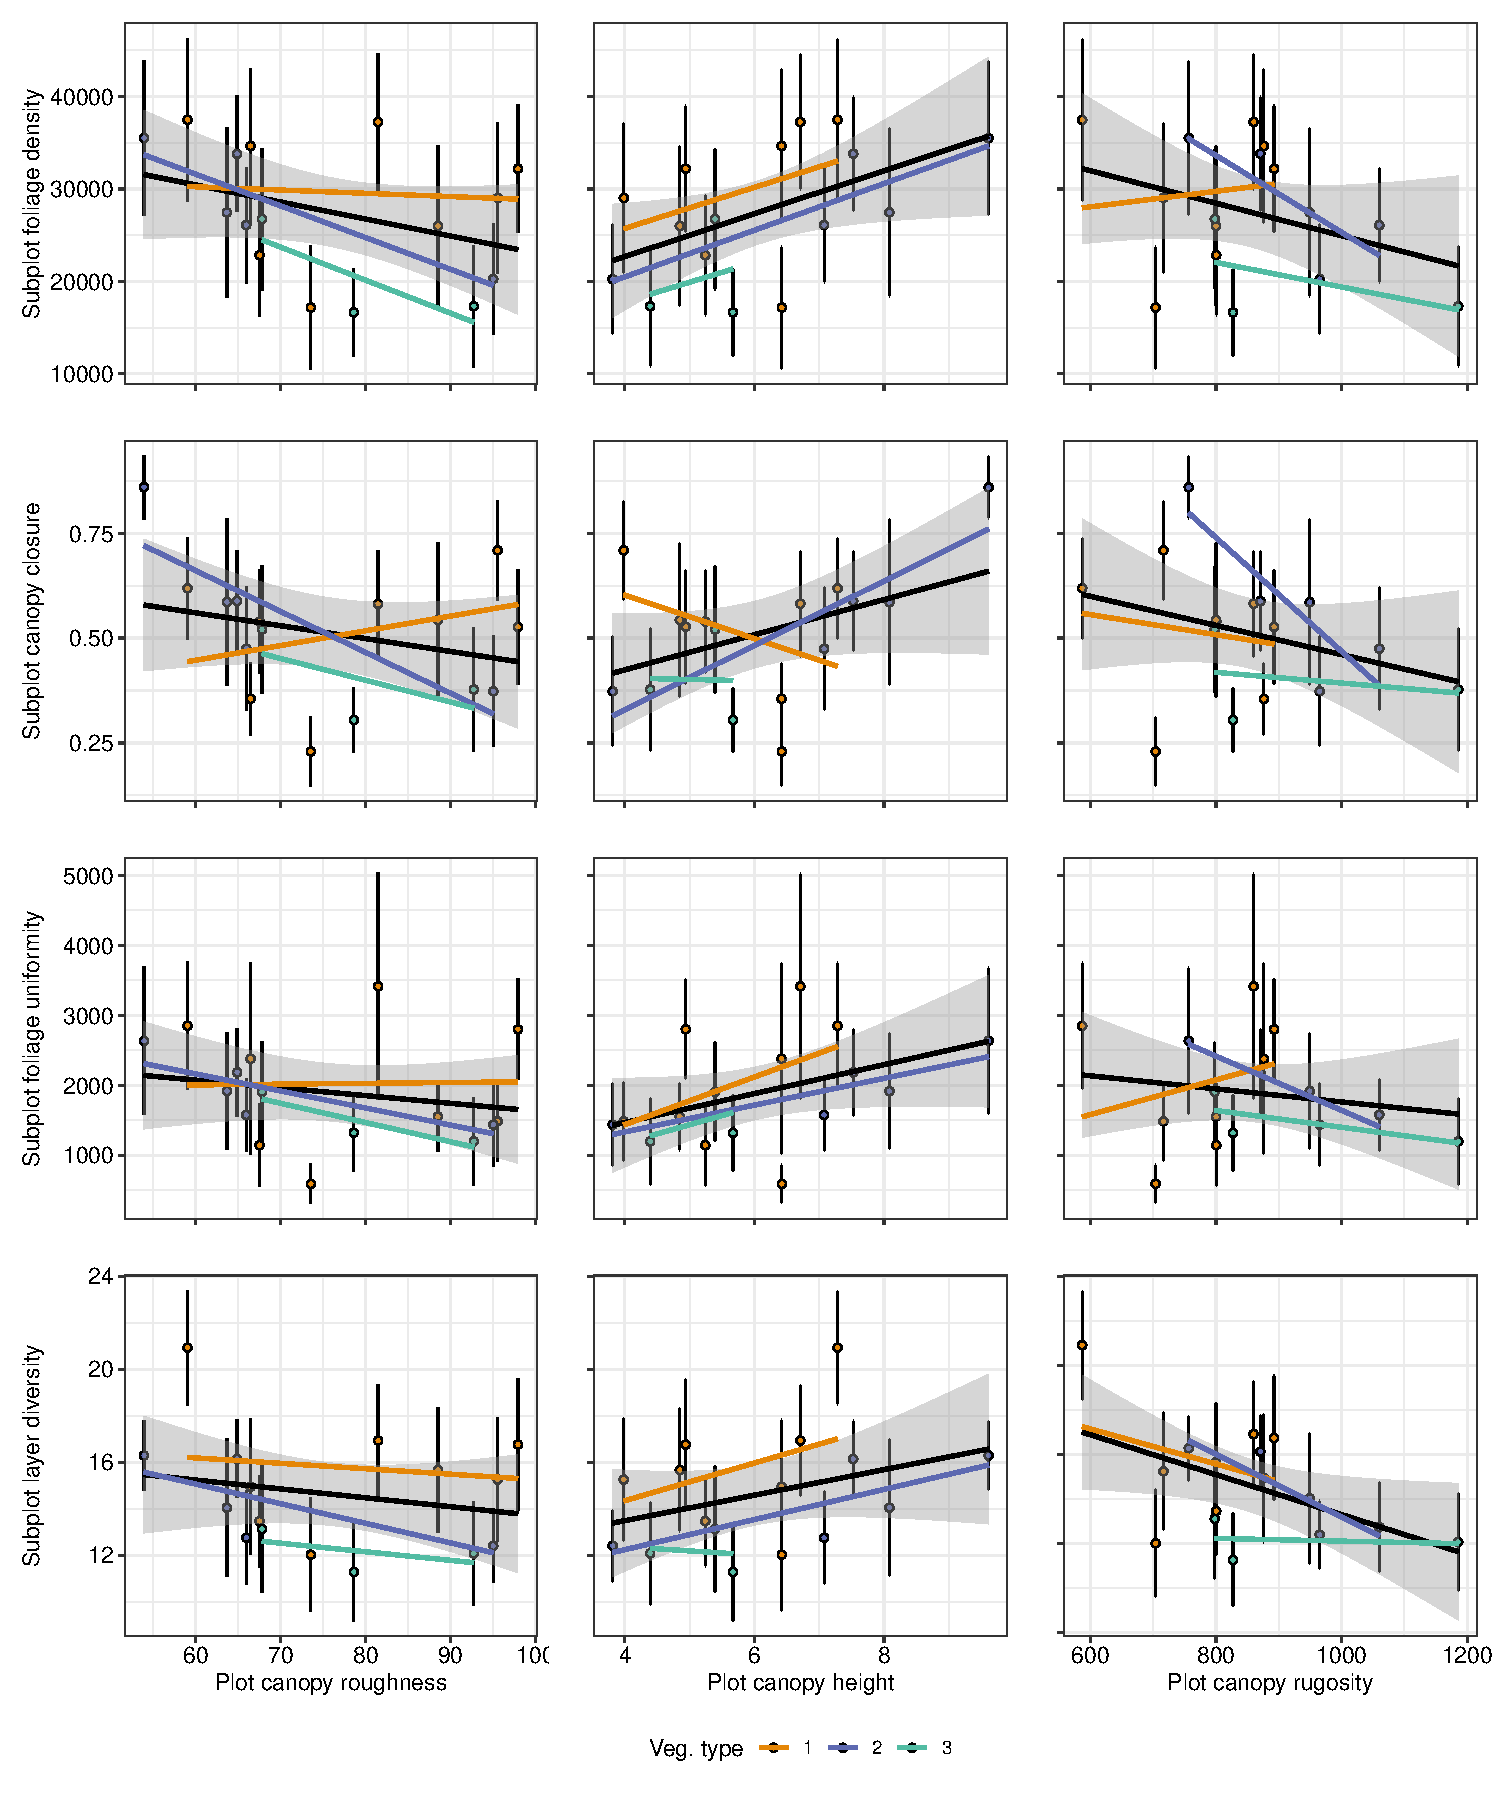
\includegraphics[width=\linewidth]{plot_subplot_bivar}
	\caption{Bivariate plots of canopy structural metrics at the subplot (y axis) and plot level (x axis). Each point represents the mean values of a single plot. Points and linear model fits are coloured according to vegetation type. The black linear model combines all vegetation types. Error bars on points are the standard deviation of mean subplot metrics across the plot.}
	\label{plot_subplot_bivar}
\end{figure}

\section{Discussion}

We investigated the effects of tree species diversity and structural diversity on several metrics of canopy complexity that were hypothesised to affect plot productivity. Species diversity appeared to generally have weak positive effects on canopy complexity at both the subplot and plot scales, while stand structural diversity had much stronger effects. The strongest determinant of canopy complexity was stem crowding, as measured by basal area and the Hegyi crowding index.

The positive relationships between species richness and subplot canopy complexity metrics observed in the subplot bivariate models were not seen in the linear mixed effects models. This is likely because the observed species richness effect was itself driven by stand structure. The Hegyi crowding index increases with stem density, i.e. decreased distance of individuals from the subplot centre. Species richness also increases with stem density, as a greater number of individuals is more likely to hold more species simply through sampling effects. \citet{Jucker2015} however, did find that increased species diversity led to greater canopy packing in European forests, with trees in mixed forests having generally larger crowns. Our result that species diversity did not have consistent effects on canopy complexity may be specific to the vegetation type studied here. Southern African open woodlands are much more heavily affected by disturbance from fire and herbivory than temperate forests, meaning the effects of inter-specific competition are weakened as a driver of stand and canopy structure \citep{}.

Canopy structure at the plot level was less well predicted by stand structure and species diversity than subplot level canopy structure. Results at the plot level suggest that woodland vegetation type and basal area has the greatest effect on canopy complexity. The two thorny savanna plots in Mtarure produced strong positive effects of basal area and diameter variantion on canopy closure, canopy height, and canopy roughness, but when these plots are removed the remaining points do not produce strong relationships. 

Facilitation might be more important in these woodlands than in temperate woodlands. Large canopy trees may cause micro-climate amelioration for understorey saplings, protecting them from drying conditions caused by the sun and wind. Facilitation has been under-played in BEFR research \citep{Wright2021}.

Scheuermann2018
Canopy rugosity didn't vary regardless of the LAI and species diversity - it just increased linearly throughout succession, for the first 100 years before becoming stable.

A more heterogeneous vegetation arrangement allows for deeper light vegetation into the canopy and when paired with a higher LAI lead to greater light interception by the subcanopy, and thus the canopy as a whole.

NPP may increase with increased canopy heterogeneity, because subcanopy plants are normally light limited and sensitive to small increases in available light such as those provided by deeper light penetration in a heterogenous canopy.

Fotis2017
Hardiman et al. 2011, 2013a, found that increased rugosity in the canopy increased NPP in temperature forests. Fahey et al. 2015 in an old-growth forest.

Canopy structure can affect canopy-level photosynthesis (Kira et al. 1969, Chen et al. 2012), light-use efficiency (Walcroft et al. 2005, Duursma and Makela 2007) and NEE (Baldochii and Wilson 2001, Law et al. 2001) through its influence on both total light interception and its variability within the canopy.

While other studies have found links between light environment and canopy structure, in our sites maybe the canopy is too sparse for this to be an issue.

Shirima2015
* In Miombo woodlands, AGB higher under denser vegetation canopies
	* Maybe the canopy provides amelioration of harsher environmental conditions in this system


\section{Conclusion}

\printbibliography

%\section{Supplementary Material} \beginsupplement

% latex table generated in R 4.1.0 by xtable 1.8-4 package
% Thu Aug 12 16:12:36 2021
\begin{longtable}{llccccS[table-format=-2.2, table-space-text-post = {***}]}
\caption{Summary statistics of bivariate linear models comparing canopy complexity metrics with diversity and stand structural metrics. Slope refers to the slope of the predictor term in the model, $\pm{}$ 1 standard error. R\textsuperscript{2} refers to the whole model. T is the t-value of the slope of the predictor term in the model, Asterisks indicate the p-value of these terms (***<0.001, **<0.01, *<0.05).} \\ 
  \toprule
{Response} & {Predictor} & {Cluster} & {Slope} & {F} & {R\textsuperscript{2}} & {T} \\ 
  \midrule
{\multirow{5}{*}{Foliage density}} & {\multirow{5}{*}{Basal area CoV}} & 1 &  5.3e+01$\pm$2.9e+01 & 3.4(2,97) & 0.03 & 1.85 \\ 
   &  & 2 &  1.4e+02$\pm$4.9e+01 & 8.5(2,38) & 0.18 & 2.92** \\ 
   &  & 3 &  9.5e+01$\pm$6.4e+01 & 2.2(2,14) & 0.14 & 1.49 \\ 
   &  & 4 & -1.7e+02$\pm$1.4e+02 & 1.5(2,12) & 0.11 & -1.21 \\ 
   &  & All &  8.0e+01$\pm$2.3e+01 & 12.5(2,167) & 0.07 & 3.53*** \\ 
   \midrule
{\multirow{5}{*}{Foliage density}} & {\multirow{5}{*}{Hegyi}} & 1 &  6.2e+03$\pm$1.6e+03 & 15.5(2,102) & 0.13 & 3.93*** \\ 
   &  & 2 &  1.1e+04$\pm$2.3e+03 & 22.0(2,40) & 0.36 & 4.69*** \\ 
   &  & 3 &  1.0e+04$\pm$2.4e+03 & 17.7(2,23) & 0.43 & 4.21*** \\ 
   &  & 4 &  4.1e+03$\pm$4.0e+03 & 1.0(2,13) & 0.07 & 1.02 \\ 
   &  & All &  8.2e+03$\pm$1.1e+03 & 50.7(2,184) & 0.22 & 7.12*** \\ 
   \midrule
{\multirow{5}{*}{Foliage density}} & {\multirow{5}{*}{Richness}} & 1 &  2.3e+03$\pm$8.8e+02 & 7.1(2,102) & 0.07 & 2.67** \\ 
   &  & 2 &  3.1e+03$\pm$1.3e+03 & 6.0(2,40) & 0.13 & 2.45* \\ 
   &  & 3 &  1.2e+04$\pm$3.6e+03 & 11.7(2,23) & 0.34 & 3.43** \\ 
   &  & 4 & -1.8e+03$\pm$3.9e+03 & 0.2(2,13) & 0.02 & -0.46 \\ 
   &  & All &  3.1e+03$\pm$6.7e+02 & 20.8(2,184) & 0.10 & 4.57*** \\ 
   \midrule
{\multirow{5}{*}{Canopy closure}} & {\multirow{5}{*}{Basal area CoV}} & 1 &  1.3e-04$\pm$5.4e-04 & 0.1(2,97) & 0.00 & 0.24 \\ 
   &  & 2 &  2.7e-03$\pm$1.0e-03 & 7.3(2,39) & 0.16 & 2.70* \\ 
   &  & 3 &  3.7e-03$\pm$9.7e-04 & 14.3(2,14) & 0.50 & 3.78** \\ 
   &  & 4 & -4.3e-03$\pm$2.8e-03 & 2.3(2,12) & 0.16 & -1.53 \\ 
   &  & All &  1.1e-03$\pm$4.4e-04 & 6.5(2,168) & 0.04 & 2.55* \\ 
   \midrule
{\multirow{5}{*}{Canopy closure}} & {\multirow{5}{*}{Hegyi}} & 1 &  2.0e-01$\pm$2.4e-02 & 71.2(2,102) & 0.41 & 8.44*** \\ 
   &  & 2 &  2.5e-01$\pm$4.6e-02 & 28.8(2,41) & 0.41 & 5.37*** \\ 
   &  & 3 &  2.5e-01$\pm$3.5e-02 & 52.4(2,23) & 0.69 & 7.24*** \\ 
   &  & 4 &  1.8e-01$\pm$7.1e-02 & 6.4(2,13) & 0.33 & 2.52* \\ 
   &  & All &  2.2e-01$\pm$1.8e-02 & 148.0(2,185) & 0.44 & 12.16*** \\ 
   \midrule
{\multirow{5}{*}{Canopy closure}} & {\multirow{5}{*}{Richness}} & 1 &  1.8e-02$\pm$1.7e-02 & 1.1(2,102) & 0.01 & 1.06 \\ 
   &  & 2 &  9.2e-02$\pm$2.4e-02 & 14.7(2,41) & 0.26 & 3.83*** \\ 
   &  & 3 &  1.6e-01$\pm$8.1e-02 & 3.9(2,23) & 0.14 & 1.97 \\ 
   &  & 4 &  7.5e-02$\pm$7.9e-02 & 0.9(2,13) & 0.06 & 0.95 \\ 
   &  & All &  5.3e-02$\pm$1.3e-02 & 16.9(2,185) & 0.08 & 4.11*** \\ 
   \midrule
{\multirow{5}{*}{Foliage uniformity}} & {\multirow{5}{*}{Basal area CoV}} & 1 &  1.7e+00$\pm$3.5e+00 & 0.2(2,97) & 0.00 & 0.50 \\ 
   &  & 2 &  8.0e+00$\pm$5.4e+00 & 2.2(2,38) & 0.05 & 1.48 \\ 
   &  & 3 &  3.1e+00$\pm$6.7e+00 & 0.2(2,14) & 0.02 & 0.46 \\ 
   &  & 4 & -8.7e+00$\pm$9.4e+00 & 0.9(2,12) & 0.07 & -0.93 \\ 
   &  & All &  3.7e+00$\pm$2.5e+00 & 2.1(2,167) & 0.01 & 1.44 \\ 
   \midrule
{\multirow{5}{*}{Foliage uniformity}} & {\multirow{5}{*}{Hegyi}} & 1 &  3.1e+02$\pm$2.0e+02 & 2.4(2,102) & 0.02 & 1.56 \\ 
   &  & 2 &  4.9e+02$\pm$2.8e+02 & 3.0(2,40) & 0.07 & 1.72 \\ 
   &  & 3 &  8.3e+02$\pm$2.4e+02 & 12.0(2,23) & 0.34 & 3.46** \\ 
   &  & 4 &  2.5e+02$\pm$2.6e+02 & 0.9(2,13) & 0.07 & 0.96 \\ 
   &  & All &  4.7e+02$\pm$1.3e+02 & 12.5(2,184) & 0.06 & 3.53*** \\ 
   \midrule
{\multirow{5}{*}{Foliage uniformity}} & {\multirow{5}{*}{Richness}} & 1 &  2.1e+02$\pm$1.1e+02 & 3.8(2,102) & 0.04 & 1.96 \\ 
   &  & 2 &  1.3e+02$\pm$1.3e+02 & 1.0(2,40) & 0.02 & 0.98 \\ 
   &  & 3 &  1.3e+03$\pm$3.1e+02 & 17.4(2,23) & 0.43 & 4.18*** \\ 
   &  & 4 & -1.1e+02$\pm$2.5e+02 & 0.2(2,13) & 0.01 & -0.44 \\ 
   &  & All &  2.2e+02$\pm$7.3e+01 & 8.8(2,184) & 0.05 & 2.97** \\ 
   \midrule
{\multirow{5}{*}{Layer diversity}} & {\multirow{5}{*}{Basal area CoV}} & 1 &  2.5e-02$\pm$9.3e-03 & 7.1(2,97) & 0.07 & 2.66** \\ 
   &  & 2 &  3.9e-02$\pm$1.4e-02 & 8.0(2,38) & 0.17 & 2.83** \\ 
   &  & 3 &  2.7e-02$\pm$2.3e-02 & 1.3(2,14) & 0.09 & 1.15 \\ 
   &  & 4 &  2.1e-02$\pm$3.1e-02 & 0.5(2,12) & 0.04 & 0.67 \\ 
   &  & All &  3.2e-02$\pm$7.6e-03 & 17.6(2,167) & 0.10 & 4.20*** \\ 
   \midrule
{\multirow{5}{*}{Layer diversity}} & {\multirow{5}{*}{Hegyi}} & 1 &  2.7e+00$\pm$4.9e-01 & 29.1(2,102) & 0.22 & 5.39*** \\ 
   &  & 2 &  2.0e+00$\pm$7.5e-01 & 7.1(2,40) & 0.15 & 2.66* \\ 
   &  & 3 &  1.9e+00$\pm$1.0e+00 & 3.6(2,23) & 0.13 & 1.89 \\ 
   &  & 4 &  1.1e+00$\pm$8.5e-01 & 1.8(2,13) & 0.12 & 1.33 \\ 
   &  & All &  2.7e+00$\pm$3.9e-01 & 46.8(2,184) & 0.20 & 6.84*** \\ 
   \midrule
{\multirow{5}{*}{Layer diversity}} & {\multirow{5}{*}{Richness}} & 1 &  1.0e+00$\pm$2.8e-01 & 12.5(2,102) & 0.11 & 3.54*** \\ 
   &  & 2 &  7.0e-01$\pm$3.6e-01 & 3.8(2,40) & 0.09 & 1.94 \\ 
   &  & 3 &  3.8e+00$\pm$1.3e+00 & 8.8(2,23) & 0.28 & 2.97** \\ 
   &  & 4 &  5.7e-01$\pm$8.4e-01 & 0.5(2,13) & 0.03 & 0.68 \\ 
   &  & All &  1.1e+00$\pm$2.2e-01 & 24.3(2,184) & 0.12 & 4.93*** \\ 
   \midrule
{\multirow{5}{*}{Canopy roughness}} & {\multirow{5}{*}{Basal area CoV}} & 1 &  1.2e-01$\pm$6.9e-02 & 2.9(2,6) & 0.33 & 1.72 \\ 
   &  & 2 & -3.2e-01$\pm$2.9e-01 & 1.2(2,3) & 0.29 & -1.10 \\ 
   &  & 3 &  3.5e-01$\pm$4.7e-01 & 0.6(2,1) & 0.36 & 0.74 \\ 
   &  & 4 &  &  &  &  \\ 
   &  & All &  3.0e-02$\pm$5.0e-02 & 0.4(2,16) & 0.02 & 0.60 \\ 
   \midrule
{\multirow{5}{*}{Canopy roughness}} & {\multirow{5}{*}{Mingling}} & 1 & -4.2e+01$\pm$5.7e+01 & 0.5(2,6) & 0.08 & -0.74 \\ 
   &  & 2 &  1.6e+01$\pm$9.7e+01 & 0.0(2,3) & 0.01 & 0.17 \\ 
   &  & 3 &  3.5e+02$\pm$2.5e+02 & 2.0(2,1) & 0.67 & 1.42 \\ 
   &  & 4 &  &  &  &  \\ 
   &  & All & -2.8e+01$\pm$3.3e+01 & 0.7(2,16) & 0.04 & -0.86 \\ 
   \midrule
{\multirow{5}{*}{Canopy roughness}} & {\multirow{5}{*}{Richness}} & 1 & -1.8e+00$\pm$1.6e+00 & 1.1(2,6) & 0.16 & -1.06 \\ 
   &  & 2 & -1.2e+00$\pm$4.6e-01 & 6.5(2,3) & 0.68 & -2.55 \\ 
   &  & 3 & -5.4e+00$\pm$1.1e+01 & 0.2(2,1) & 0.19 & -0.48 \\ 
   &  & 4 &  &  &  &  \\ 
   &  & All & -9.0e-01$\pm$3.2e-01 & 7.8(2,16) & 0.33 & -2.79* \\ 
   \midrule
{\multirow{5}{*}{Canopy roughness}} & {\multirow{5}{*}{Tree density}} & 1 & -4.3e-02$\pm$4.5e-02 & 0.9(2,6) & 0.13 & -0.96 \\ 
   &  & 2 & -5.9e-02$\pm$3.1e-02 & 3.6(2,3) & 0.54 & -1.89 \\ 
   &  & 3 & -1.8e-01$\pm$2.6e-01 & 0.5(2,1) & 0.31 & -0.68 \\ 
   &  & 4 &  &  &  &  \\ 
   &  & All & -2.6e-02$\pm$1.7e-02 & 2.3(2,16) & 0.12 & -1.51 \\ 
   \midrule
{\multirow{5}{*}{Canopy roughness}} & {\multirow{5}{*}{Winkelmass}} & 1 & -7.3e+01$\pm$2.6e+02 & 0.1(2,6) & 0.01 & -0.29 \\ 
   &  & 2 &  6.6e+02$\pm$5.0e+02 & 1.7(2,3) & 0.37 & 1.32 \\ 
   &  & 3 &  2.3e+02$\pm$4.2e+02 & 0.3(2,1) & 0.23 & 0.54 \\ 
   &  & 4 &  &  &  &  \\ 
   &  & All &  1.8e+02$\pm$1.6e+02 & 1.3(2,16) & 0.08 & 1.14 \\ 
   \midrule
{\multirow{5}{*}{Canopy height}} & {\multirow{5}{*}{Basal area CoV}} & 1 & -6.5e-03$\pm$6.1e-03 & 1.1(2,6) & 0.16 & -1.07 \\ 
   &  & 2 &  4.3e-02$\pm$4.0e-02 & 1.2(2,3) & 0.28 & 1.08 \\ 
   &  & 3 & -3.1e-02$\pm$8.7e-03 & 12.3(2,1) & 0.92 & -3.51 \\ 
   &  & 4 &  &  &  &  \\ 
   &  & All &  7.1e-03$\pm$7.3e-03 & 0.9(2,16) & 0.06 & 0.97 \\ 
   \midrule
{\multirow{5}{*}{Canopy height}} & {\multirow{5}{*}{Mingling}} & 1 &  6.8e+00$\pm$3.8e+00 & 3.2(2,6) & 0.34 & 1.78 \\ 
   &  & 2 & -3.3e+00$\pm$1.3e+01 & 0.1(2,3) & 0.02 & -0.25 \\ 
   &  & 3 & -2.3e+01$\pm$9.3e-01 & 619.2(2,1) & 1.00 & -24.88* \\ 
   &  & 4 &  &  &  &  \\ 
   &  & All &  3.8e+00$\pm$4.8e+00 & 0.6(2,16) & 0.04 & 0.79 \\ 
   \midrule
{\multirow{5}{*}{Canopy height}} & {\multirow{5}{*}{Richness}} & 1 &  9.2e-02$\pm$1.4e-01 & 0.4(2,6) & 0.07 & 0.67 \\ 
   &  & 2 &  1.7e-01$\pm$5.7e-02 & 8.6(2,3) & 0.74 & 2.94 \\ 
   &  & 3 & -1.4e-01$\pm$6.6e-01 & 0.0(2,1) & 0.04 & -0.21 \\ 
   &  & 4 &  &  &  &  \\ 
   &  & All &  1.6e-01$\pm$4.3e-02 & 13.2(2,16) & 0.45 & 3.63** \\ 
   \midrule
{\multirow{5}{*}{Canopy height}} & {\multirow{5}{*}{Tree density}} & 1 & -3.5e-04$\pm$3.8e-03 & 0.0(2,6) & 0.00 & -0.09 \\ 
   &  & 2 &  8.6e-03$\pm$4.0e-03 & 4.7(2,3) & 0.61 & 2.16 \\ 
   &  & 3 & -1.0e-03$\pm$1.7e-02 & 0.0(2,1) & 0.00 & -0.06 \\ 
   &  & 4 &  &  &  &  \\ 
   &  & All &  4.3e-03$\pm$2.5e-03 & 3.1(2,16) & 0.16 & 1.76 \\ 
   \midrule
{\multirow{5}{*}{Canopy height}} & {\multirow{5}{*}{Winkelmass}} & 1 &  1.6e+01$\pm$1.9e+01 & 0.7(2,6) & 0.11 & 0.85 \\ 
   &  & 2 & -1.0e+02$\pm$6.3e+01 & 2.5(2,3) & 0.46 & -1.58 \\ 
   &  & 3 &  4.0e+00$\pm$2.5e+01 & 0.0(2,1) & 0.02 & 0.16 \\ 
   &  & 4 &  &  &  &  \\ 
   &  & All & -1.9e+01$\pm$2.3e+01 & 0.6(2,16) & 0.04 & -0.80 \\ 
   \midrule
{\multirow{5}{*}{Canopy closure}} & {\multirow{5}{*}{Basal area CoV}} & 1 &  3.1e-04$\pm$6.2e-04 & 0.3(2,10) & 0.02 & 0.50 \\ 
   &  & 2 &  3.1e-03$\pm$3.6e-03 & 0.8(2,3) & 0.21 & 0.88 \\ 
   &  & 3 &  1.5e-03$\pm$5.0e-03 & 0.1(2,1) & 0.09 & 0.31 \\ 
   &  & 4 &  &  &  &  \\ 
   &  & All &  8.4e-04$\pm$5.4e-04 & 2.4(2,20) & 0.11 & 1.56 \\ 
   \midrule
{\multirow{5}{*}{Canopy closure}} & {\multirow{5}{*}{Mingling}} & 1 & -9.1e-02$\pm$4.6e-01 & 0.0(2,10) & 0.00 & -0.20 \\ 
   &  & 2 & -6.4e-01$\pm$1.1e+00 & 0.4(2,3) & 0.11 & -0.60 \\ 
   &  & 3 & -7.5e-02$\pm$3.8e+00 & 0.0(2,1) & 0.00 & -0.02 \\ 
   &  & 4 &  &  &  &  \\ 
   &  & All &  2.8e-02$\pm$3.5e-01 & 0.0(2,20) & 0.00 & 0.08 \\ 
   \midrule
{\multirow{5}{*}{Canopy closure}} & {\multirow{5}{*}{Richness}} & 1 &  6.5e-03$\pm$1.6e-02 & 0.2(2,10) & 0.02 & 0.40 \\ 
   &  & 2 &  1.5e-02$\pm$3.6e-03 & 18.1(2,3) & 0.86 & 4.25* \\ 
   &  & 3 &  1.1e-01$\pm$2.0e-02 & 28.0(2,1) & 0.97 & 5.29 \\ 
   &  & 4 &  &  &  &  \\ 
   &  & All &  1.3e-02$\pm$3.8e-03 & 11.0(2,20) & 0.35 & 3.32** \\ 
   \midrule
{\multirow{5}{*}{Canopy closure}} & {\multirow{5}{*}{Tree density}} & 1 &  1.4e-04$\pm$3.6e-04 & 0.1(2,10) & 0.01 & 0.39 \\ 
   &  & 2 &  8.6e-04$\pm$2.1e-04 & 17.6(2,3) & 0.85 & 4.20* \\ 
   &  & 3 &  2.8e-03$\pm$1.1e-04 & 634.0(2,1) & 1.00 & 25.18* \\ 
   &  & 4 &  &  &  &  \\ 
   &  & All &  4.8e-04$\pm$1.7e-04 & 7.8(2,20) & 0.28 & 2.80* \\ 
   \midrule
{\multirow{5}{*}{Canopy closure}} & {\multirow{5}{*}{Winkelmass}} & 1 & -3.6e+00$\pm$2.1e+00 & 3.0(2,10) & 0.23 & -1.72 \\ 
   &  & 2 & -1.1e+01$\pm$3.2e+00 & 12.7(2,3) & 0.81 & -3.56* \\ 
   &  & 3 & -4.1e+00$\pm$5.7e-01 & 53.4(2,1) & 0.98 & -7.30 \\ 
   &  & 4 &  &  &  &  \\ 
   &  & All & -4.0e+00$\pm$1.6e+00 & 6.0(2,20) & 0.23 & -2.45* \\ 
   \midrule
{\multirow{5}{*}{Canopy rugosity}} & {\multirow{5}{*}{Basal area CoV}} & 1 & -1.0e-01$\pm$6.1e-01 & 0.0(2,6) & 0.00 & -0.17 \\ 
   &  & 2 & -2.2e+00$\pm$2.2e+00 & 1.1(2,3) & 0.26 & -1.03 \\ 
   &  & 3 &  8.7e+00$\pm$5.4e+00 & 2.6(2,1) & 0.73 & 1.62 \\ 
   &  & 4 &  &  &  &  \\ 
   &  & All & -1.0e+00$\pm$5.3e-01 & 3.7(2,16) & 0.19 & -1.92 \\ 
   \midrule
{\multirow{5}{*}{Canopy rugosity}} & {\multirow{5}{*}{Mingling}} & 1 & -5.9e+02$\pm$3.6e+02 & 2.7(2,6) & 0.31 & -1.63 \\ 
   &  & 2 &  8.5e+02$\pm$5.2e+02 & 2.7(2,3) & 0.47 & 1.63 \\ 
   &  & 3 &  7.2e+03$\pm$1.7e+03 & 17.6(2,1) & 0.95 & 4.19 \\ 
   &  & 4 &  &  &  &  \\ 
   &  & All &  1.3e+02$\pm$3.8e+02 & 0.1(2,16) & 0.01 & 0.33 \\ 
   \midrule
{\multirow{5}{*}{Canopy rugosity}} & {\multirow{5}{*}{Richness}} & 1 & -2.6e+01$\pm$7.5e+00 & 12.3(2,6) & 0.67 & -3.51* \\ 
   &  & 2 & -6.9e+00$\pm$4.5e+00 & 2.4(2,3) & 0.45 & -1.56 \\ 
   &  & 3 & -1.5e+01$\pm$2.2e+02 & 0.0(2,1) & 0.00 & -0.07 \\ 
   &  & 4 &  &  &  &  \\ 
   &  & All & -6.7e+00$\pm$4.2e+00 & 2.5(2,16) & 0.13 & -1.58 \\ 
   \midrule
{\multirow{5}{*}{Canopy rugosity}} & {\multirow{5}{*}{Tree density}} & 1 & -1.9e-01$\pm$3.4e-01 & 0.3(2,6) & 0.05 & -0.56 \\ 
   &  & 2 & -4.6e-01$\pm$2.1e-01 & 4.9(2,3) & 0.62 & -2.22 \\ 
   &  & 3 & -1.2e+00$\pm$5.4e+00 & 0.0(2,1) & 0.05 & -0.22 \\ 
   &  & 4 &  &  &  &  \\ 
   &  & All & -5.2e-01$\pm$1.7e-01 & 10.0(2,16) & 0.38 & -3.16** \\ 
   \midrule
{\multirow{5}{*}{Canopy rugosity}} & {\multirow{5}{*}{Winkelmass}} & 1 & -2.6e+03$\pm$1.5e+03 & 3.0(2,6) & 0.33 & -1.73 \\ 
   &  & 2 &  6.8e+03$\pm$2.4e+03 & 8.3(2,3) & 0.73 & 2.88 \\ 
   &  & 3 &  9.7e+02$\pm$8.2e+03 & 0.0(2,1) & 0.01 & 0.12 \\ 
   &  & 4 &  &  &  &  \\ 
   &  & All & -1.4e+03$\pm$1.8e+03 & 0.6(2,16) & 0.03 & -0.75 \\ 
   \bottomrule
\label{bivar_lm_summ}
\end{longtable}



\end{document}
